%% testunisatut.tex
%% Testing the Unisa tut letter class
%% 2020


%% WORKAROUND needed to pass colour names to xcolor package
%\PassOptionsToPackage{svgnames}{xcolor}

\documentclass{unisatut} 
%\documentclass[nomathsf]{unisatut} 
%% Use the unisatut class to create tutorial letters

%% UNISA tut letter details
\TutName        {Tutorial Letter}		% usually {Tutorial Letter}
\ModuleCode     {YUM123C}
\TutNum         {102}
\ModuleSemester {1}
\ModuleYear     {2021}
\ModuleName     {Cheese Making}
\Department     {Silly Walks}
\School         {Fish}
\Content        {This document tests the basics of the unisatut.sty document class.}

%% INPUT pre-defined things that get used often
%% LaTeX oreamble to include in all UNISA tut letters
%%

%% SET path to graphics
\graphicspath{ {./} }
%\graphicspath{ {./images/} }


%% LOAD packages and set options

\usepackage{
	acronym,
	amsfonts,  			% blackboard bold symbols e.g. for real numbers
	amsmath,			% for any decent maths
	amssymb,			% AMS symbols
    array,			
	comment,			% selective in/exclusion of text
	enumitem,
%	etoolbox,			% e_Tex toolbox
	framed,             % nicer frames
	gensymb,
	graphicx,  			% include jpeg or pdf pictures
%	hyperref,			% to use URLs in the text
%	ifthen,				% logical flow control
    karnaugh-map, 		% Karnaugh maps
	lineno,				% add line numbers to text
	listings,           % to show code listings
	longtable,			% multi-page tables
	mathtools,			% ditto
	microtype,			% perform various microtypesetting tricks
    pgfmath,
	subfigure,			% multiple figures in one
	textcomp,
	tikz,				% Tikz figures and diagrams
	tikz-3dplot,		% 3D plots in Tikz
%	verbatim,			% verbatim text and multiline comments
	wrapfig,			% wrap text around figures
	xcolor,             % pre-defined colour names
	xfrac,				% better-looking fractions - uses \sfrac
	}

\usepackage[
    colorlinks=true,    % use coloured hyperlinks
    breaklinks=true,    % break links across lines
    ]{hyperref}




%% ADJUST some dimensions

%% add space between paragraphs
\setlength{\parskip}{12pt plus6pt minus4pt}




%% DEFINE new commands or re-define existing commmands

%% red line across page to use as editing marker
\newcommand{\redline}{
\textcolor{red}{\noindent\makebox[\linewidth]{\rule{\paperwidth}{10pt}}}}

%% thin black line across the width of the text
\newcommand{\textwidthline}{
\noindent\makebox[\linewidth]{\rule{\textwidth}{0.4pt}}}


%% command to add an open line
\def\wl{\par \vspace{\baselineskip}}

%% 
\newcommand{\var}[2]{% 
   \newlength{#1} 
   \setlength{#1}{#2} 
} 





%% DEFINE specific colour names
\definecolor{colour_coffee}{RGB}{219,144,71}
\definecolor{colour_airforceblue}{RGB}{0.36, 0.54, 0.66}
\definecolor{shadecolor}{rgb}{1.0,0.8,0.3}





%% TIKZ stuff

%% TIKZ libraries to load
\usetikzlibrary{
    automata,
    shapes,
    shapes.geometric,
    shapes.callouts,
    patterns,
    calc,
    intersections,
    angles,
    quotes,
    arrows.meta,
    arrows,
    decorations,
      decorations.markings,
      decorations.text,
      decorations.pathmorphing,
    positioning,
    }


%% set up TIKZ values and styles
\tikzset{
%% global TIKZ settings
	x=1cm,
	y=1cm,
	axis/.style={
		very thick,
		-latex,
		>=stealth'
	},
%% arrow to use in graphs
	grapharrow/.style={
		-latex,
		>=stealth'
	},
%% red triangle with black border
	triangle/.style={
		line width=0.5pt,
		draw=black,
		fill=red!60,
		shape border rotate=#1,
		isosceles triangle,
		isosceles triangle apex angle=60,
		minimum height=0.2cm,
		minimum width=0.25cm,
		isosceles triangle stretches,
		inner sep=0pt
	},
%% thin axis
	thinaxis/.style={
		thick
	},
%% black triangle
	triangle/.style={
		line width=0.3pt,
		draw=black,
		shape border rotate=#1,
		isosceles triangle,
		isosceles triangle apex angle=60,
		minimum height=0.2cm,
		minimum width=0.25cm,
%		isosceles triangle stretches,
		inner sep=0pt
	},
%% triangle with point up
	trianglepointup/.style={
		triangle=+90
		},
%% triangle with point down
	trianglepointdown/.style={
		triangle=-90
	},
%% node representing negative values
	negnode/.style={
		trianglepointdown,
		fill=red!60
	},
%% node representing positive values
	posnode/.style={
		line width=0.5pt,
		draw=black,
		fill=green!60,
		rectangle,
		minimum height=0.2cm,
		minimum width=0.2cm,
		inner sep=0pt
	},
%% node representing hypothesis in decision tree learning
	hypothesis/.style={
		rectangle,
%		fill=blue!10,
		inner sep=1pt,
		minimum size=4mm
	},
%% empty node
	nodenoborder/.style={
		rectangle,
%		fill=blue!10,
		inner sep=1pt,
		minimum size=4mm
	},
%% decision tree node
	dectreenode/.style={
		rectangle,
		draw=black,
		line width=0.75pt,
		fill=white,
		inner sep=2pt,
		minimum height=0.5cm
	},
%% decision node
    decnode/.style={
        circle,
        draw=black,
        line width=0.75pt,
        fill=white,
        inner sep=1pt,
        minimum size=0.8cm
    },
%% leaf node in graph
	leafnode/.style={
		rectangle,
		draw=black,
		line width=0.75pt,
		fill=white,
		rounded corners=1mm,
		inner sep=1pt,
		minimum size=0.8cm
	},
%% leaf node in decision tree
	leaftreenode/.style={
		rectangle,
%		draw=black,
%		line width=0.75pt,
		fill=white,
%		rounded corners=1mm,
		inner sep=2pt,
		minimum size=0.8cm
	},
%% full line arc in decision tree
	decarrowfull/.style={
		-latex,
		>=stealth',
		line width=1.2pt
	},
%% dashed line arc in decision tree
	decarrowdashed/.style={
		-latex,
		>=stealth',
		dashed,
		line width=1.2pt,
	},
%% dotted arrow
	arrowdotted/.style={
		-latex,
		>=stealth',
		dotted,
		line width=1.2pt,
	},
%% speech bubble for comments or details in diagrams
	notice/.style={
		draw,
		fill=yellow!30,
		rectangle callout,
%		callout relative pointer={#1}
		callout absolute pointer={#1}
	},
%% vector
	vecarrow/.style={
		line width=3pt,
		decoration={markings,mark=at position 1 with 
			{\arrow[line width = 3pt,fill=white]{open triangle 60}}},
		double distance=0.0pt,
		shorten >= 5.5pt,
		preaction = {decorate},
		shorten >= 3pt,
		postaction = {
			draw,
			line width=2.5pt,
			white,
			shorten >= 15pt}
	},
%% hyperplane line for 2D neural networks 
	hyperplane/.style={
		draw=blue,
		line width=3pt,
		opacity=0.3
	},
%% node in perceptron neural network 
	perceptronnode/.style={
		circle,
		draw=black,
		line width=0.75pt,
		fill=white,
		inner sep=2pt,
		minimum size=2cm
	},
%% input node in perceptron neural network
	perceptroninput/.style={
		circle,
		draw=black,
		line width=0.75pt,
		fill=black!50,
		inner sep=0pt,
		minimum size=0.75cm
	},
%% circle node
    circnode/.style={
        line width=0.5pt,
        draw=black,
        fill=blue!60,
        circle,
        minimum height=0.2cm,
        minimum width=0.2cm,
        inner sep=0pt
    },
}



%%%%%%%%%%%%%%%%%%%%%%%%%%%%%%%%%%%%%%%%%%%%%%%%%%%








\begin{document}

%% Show line numbers - useful when commenting
%\linenumbers

\tableofcontents
\listoffigures
\listoftables


\section{INTRODUCTION}
	
This document demonstrates some aspects of the {\tt unisatut.cls} class file to create Unisa styled tutorial letters.

\subsection{Files}

The {\tt unisatut} class consists of a number of files:
\begin{itemize}
	\item{{\tt unisatut.cls} - 
					the class definition}
	\item{{\tt testunisatut.tex} - 
					the \LaTeX\ source for this document}
	\item{{\tt testunisatut.pdf} - 
					the PDF output of this document}
	\item{{\tt unisabw.eps}, {\tt unisabw.pdf}, {\tt unisabw.ps} - 
					images for use in creating the tutorial letter front page and other bits}
	\item{{\tt unisatutpreamble.tex} - 
					load generic/global packages and definitions to use in all tutorial letters}
	\item{{\tt cheeseharpers.pjg} - 
					used as an example input image in this document}
\end{itemize}


\subsection{Usage}

Copy all the files into the same directory, or somewhere in the \LaTeX path. 
You can also create a separate directory for the graphic files 
	(see {\tt unisatutpreamble.tex} on how to set the path.)

Document class definition:
\wl 

\begin{lstlisting}[frame=single]
\documentclass[options]{unisatut}
\end{lstlisting}
Options:
\begin{itemize}
	\item{{\tt nomathsf} - 
		by default, the class typesets mathematics using uses a Sans Serif font. 
		This option sets mathematics typesetting to a Serif (Roman) font.}
	\item{{\tt solution} - 
		this may not work properly, and has not been tested. 
		It is a remnant from Yorick's class that uses an {\tt assignment} environment and can include solutions.}
	\item{{\tt online} - also a remnant from the 2012 online MOOs. To be removed in a future version.}
\end{itemize}

The tutorial letter labels, such as modulecode, year, and so on, are controlled using variables defined 
	in the document preamble. 
{\tt Department} and {\tt School} are optional, and will not appear on the front page if not defined. 
The \LaTeX\ document should contain the following:
\wl

\begin{lstlisting}[frame=single]
\documentclass[nomathsf]{unisatut} 

\TutName        {Tutorial Letter}
\ModuleCode     {YUM123C}
\TutNum         {102}
\ModuleSemester {1}
\ModuleYear     {2021}
\ModuleName     {Cheese Making}
\Department     {Silly Walks}
\School         {Fish}
\Content        {This document tests the unisatut.sty document class.}

%% INPUT pre-defined things that get used often
%% LaTeX oreamble to include in all UNISA tut letters
%%

%% SET path to graphics
\graphicspath{ {./} }
%\graphicspath{ {./images/} }


%% LOAD packages and set options

\usepackage{
	acronym,
	amsfonts,  			% blackboard bold symbols e.g. for real numbers
	amsmath,			% for any decent maths
	amssymb,			% AMS symbols
    array,			
	comment,			% selective in/exclusion of text
	enumitem,
%	etoolbox,			% e_Tex toolbox
	framed,             % nicer frames
	gensymb,
	graphicx,  			% include jpeg or pdf pictures
%	hyperref,			% to use URLs in the text
%	ifthen,				% logical flow control
    karnaugh-map, 		% Karnaugh maps
	lineno,				% add line numbers to text
	listings,           % to show code listings
	longtable,			% multi-page tables
	mathtools,			% ditto
	microtype,			% perform various microtypesetting tricks
    pgfmath,
	subfigure,			% multiple figures in one
	textcomp,
	tikz,				% Tikz figures and diagrams
	tikz-3dplot,		% 3D plots in Tikz
%	verbatim,			% verbatim text and multiline comments
	wrapfig,			% wrap text around figures
	xcolor,             % pre-defined colour names
	xfrac,				% better-looking fractions - uses \sfrac
	}

\usepackage[
    colorlinks=true,    % use coloured hyperlinks
    breaklinks=true,    % break links across lines
    ]{hyperref}




%% ADJUST some dimensions

%% add space between paragraphs
\setlength{\parskip}{12pt plus6pt minus4pt}




%% DEFINE new commands or re-define existing commmands

%% red line across page to use as editing marker
\newcommand{\redline}{
\textcolor{red}{\noindent\makebox[\linewidth]{\rule{\paperwidth}{10pt}}}}

%% thin black line across the width of the text
\newcommand{\textwidthline}{
\noindent\makebox[\linewidth]{\rule{\textwidth}{0.4pt}}}


%% command to add an open line
\def\wl{\par \vspace{\baselineskip}}

%% 
\newcommand{\var}[2]{% 
   \newlength{#1} 
   \setlength{#1}{#2} 
} 





%% DEFINE specific colour names
\definecolor{colour_coffee}{RGB}{219,144,71}
\definecolor{colour_airforceblue}{RGB}{0.36, 0.54, 0.66}
\definecolor{shadecolor}{rgb}{1.0,0.8,0.3}





%% TIKZ stuff

%% TIKZ libraries to load
\usetikzlibrary{
    automata,
    shapes,
    shapes.geometric,
    shapes.callouts,
    patterns,
    calc,
    intersections,
    angles,
    quotes,
    arrows.meta,
    arrows,
    decorations,
      decorations.markings,
      decorations.text,
      decorations.pathmorphing,
    positioning,
    }


%% set up TIKZ values and styles
\tikzset{
%% global TIKZ settings
	x=1cm,
	y=1cm,
	axis/.style={
		very thick,
		-latex,
		>=stealth'
	},
%% arrow to use in graphs
	grapharrow/.style={
		-latex,
		>=stealth'
	},
%% red triangle with black border
	triangle/.style={
		line width=0.5pt,
		draw=black,
		fill=red!60,
		shape border rotate=#1,
		isosceles triangle,
		isosceles triangle apex angle=60,
		minimum height=0.2cm,
		minimum width=0.25cm,
		isosceles triangle stretches,
		inner sep=0pt
	},
%% thin axis
	thinaxis/.style={
		thick
	},
%% black triangle
	triangle/.style={
		line width=0.3pt,
		draw=black,
		shape border rotate=#1,
		isosceles triangle,
		isosceles triangle apex angle=60,
		minimum height=0.2cm,
		minimum width=0.25cm,
%		isosceles triangle stretches,
		inner sep=0pt
	},
%% triangle with point up
	trianglepointup/.style={
		triangle=+90
		},
%% triangle with point down
	trianglepointdown/.style={
		triangle=-90
	},
%% node representing negative values
	negnode/.style={
		trianglepointdown,
		fill=red!60
	},
%% node representing positive values
	posnode/.style={
		line width=0.5pt,
		draw=black,
		fill=green!60,
		rectangle,
		minimum height=0.2cm,
		minimum width=0.2cm,
		inner sep=0pt
	},
%% node representing hypothesis in decision tree learning
	hypothesis/.style={
		rectangle,
%		fill=blue!10,
		inner sep=1pt,
		minimum size=4mm
	},
%% empty node
	nodenoborder/.style={
		rectangle,
%		fill=blue!10,
		inner sep=1pt,
		minimum size=4mm
	},
%% decision tree node
	dectreenode/.style={
		rectangle,
		draw=black,
		line width=0.75pt,
		fill=white,
		inner sep=2pt,
		minimum height=0.5cm
	},
%% decision node
    decnode/.style={
        circle,
        draw=black,
        line width=0.75pt,
        fill=white,
        inner sep=1pt,
        minimum size=0.8cm
    },
%% leaf node in graph
	leafnode/.style={
		rectangle,
		draw=black,
		line width=0.75pt,
		fill=white,
		rounded corners=1mm,
		inner sep=1pt,
		minimum size=0.8cm
	},
%% leaf node in decision tree
	leaftreenode/.style={
		rectangle,
%		draw=black,
%		line width=0.75pt,
		fill=white,
%		rounded corners=1mm,
		inner sep=2pt,
		minimum size=0.8cm
	},
%% full line arc in decision tree
	decarrowfull/.style={
		-latex,
		>=stealth',
		line width=1.2pt
	},
%% dashed line arc in decision tree
	decarrowdashed/.style={
		-latex,
		>=stealth',
		dashed,
		line width=1.2pt,
	},
%% dotted arrow
	arrowdotted/.style={
		-latex,
		>=stealth',
		dotted,
		line width=1.2pt,
	},
%% speech bubble for comments or details in diagrams
	notice/.style={
		draw,
		fill=yellow!30,
		rectangle callout,
%		callout relative pointer={#1}
		callout absolute pointer={#1}
	},
%% vector
	vecarrow/.style={
		line width=3pt,
		decoration={markings,mark=at position 1 with 
			{\arrow[line width = 3pt,fill=white]{open triangle 60}}},
		double distance=0.0pt,
		shorten >= 5.5pt,
		preaction = {decorate},
		shorten >= 3pt,
		postaction = {
			draw,
			line width=2.5pt,
			white,
			shorten >= 15pt}
	},
%% hyperplane line for 2D neural networks 
	hyperplane/.style={
		draw=blue,
		line width=3pt,
		opacity=0.3
	},
%% node in perceptron neural network 
	perceptronnode/.style={
		circle,
		draw=black,
		line width=0.75pt,
		fill=white,
		inner sep=2pt,
		minimum size=2cm
	},
%% input node in perceptron neural network
	perceptroninput/.style={
		circle,
		draw=black,
		line width=0.75pt,
		fill=black!50,
		inner sep=0pt,
		minimum size=0.75cm
	},
%% circle node
    circnode/.style={
        line width=0.5pt,
        draw=black,
        fill=blue!60,
        circle,
        minimum height=0.2cm,
        minimum width=0.2cm,
        inner sep=0pt
    },
}



%%%%%%%%%%%%%%%%%%%%%%%%%%%%%%%%%%%%%%%%%%%%%%%%%%%

\begin{document}
Here be dragons!
\end{document}
\end{lstlisting}

The {\tt unisatutpreamble.tex} file can be used to define packages that are used regularly, 
	their settings, adjusting dimensions, and (re-)defining common commands.


\section{BITS FROM THE TUT101 TEMPLATE}

Here follows some bits from the standard Unisa Tut 101 template, executed in \LaTeX.


Dear Student

As part of this tutorial letter, we wish to inform you that Unisa has implemented a transformation 
	charter based on five pillars and eight dimensions. 
In response to this charter, we have also placed curriculum transformation high on the agenda. 
For your information, curriculum transformation includes the following pillars: student-centred 
	scholarship, the pedagogical renewal of teaching and assessment practices, the scholarship of 
	teaching and learning, and the infusion of African epistemologies and philosophies. 
These pillars and their principles will be integrated at both the programme and module levels, 
	as a phased-in approach. 
You will notice the implementation in your modules, and we encourage you to fully embrace these 
	changes during your studies at Unisa.  

\subsection{Getting started\ldots}

Given the nature of this module, you can read about it and find your study material online. 
Go to the website at \url{https://my.unisa.ac.za} and log in using your student number and password. 
You will see YUM123C in the row of modules displayed in the orange blocks at the top of the web page. 
Select the {\tt More} tab if you cannot find the module you require in the blocks displayed. 
Then click on the module you wish to open.
	
We wish you every success in your studies!


\section{OVERVIEW OF YUM123C}

\subsection{Purpose}

Students who have completed this module successfully will understand more about the theoretical and 
	practical aspects making their own cheese.

\subsection{Outcomes}

In this module, you will learn to do the following things:
\begin{itemize}
	\item{Describe the chemical and physical structure and properties of milk, cream, and cheese.}
	\item{Describe the genetics, physiology and biochemical processes of lactobacili.}
	\item{Learn to milk a cow.}
	\item{Learn to separate the milk into cream and whey.}
	\item{Learn to create a starter culture.}
	\item{Culture, coagulate, drain, and scald the young cheese.}
	\item{Learn patience while the mould ripens and the cheese matures.}
	\item{Appreciate the pairing of a good wine with the cheese you made.}
\end{itemize}

\newpage

\begin{wrapfigure}{l}{0.4\textwidth}
    \centering
    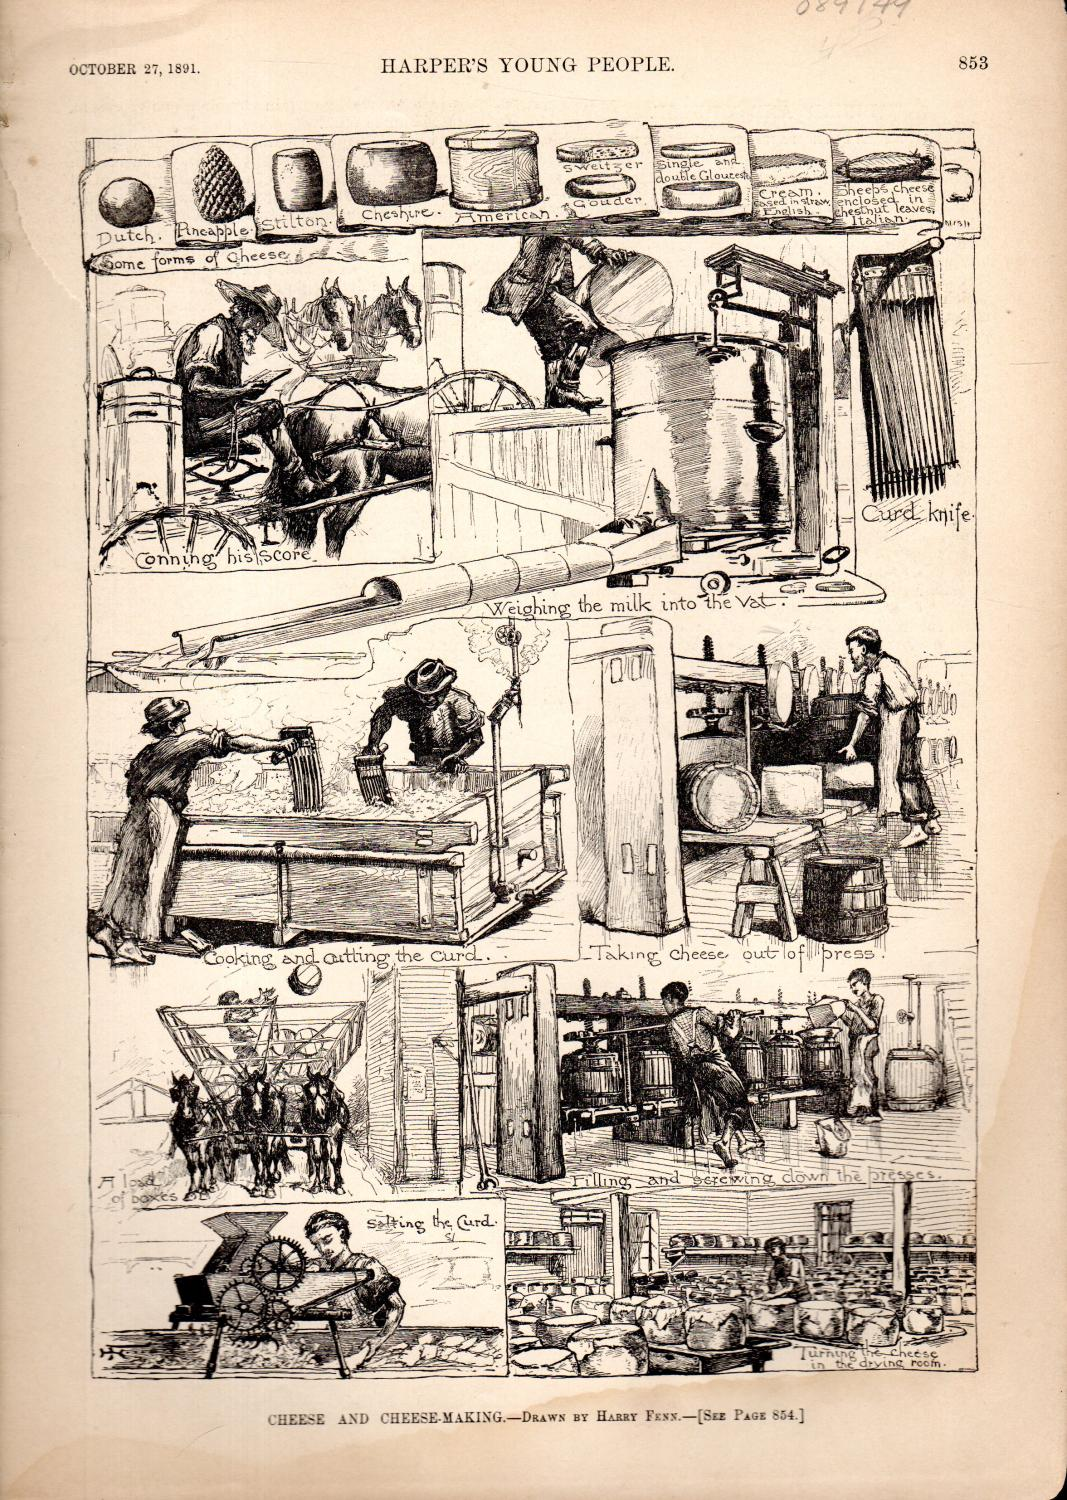
\includegraphics[width=0.4\textwidth]{cheeseharpers.jpg}
    \caption{Harper's cheesemaking.
    	{\protect\label{FIG_harperscheese}}}
\end{wrapfigure}

The image on cheese making image in Figure~\ref{FIG_harperscheese} 
	from \url{https://www.abebooks.com/servlet/BookDetailsPL?bi=30630061366}. 
The following text was liberated from Wikipedia's page on cheesemaking 
(\url{https://en.wikipedia.org/wiki/Cheesemaking}) to use as a filler.

One of the ancient cheesemakers' earliest tools for cheesemaking, cheese molds or strainers, 
	can be found throughout Europe, dating back to the Bronze Age. 
Baskets were used to separate the cheese curds, but as technology advanced, these cheese 
	molds would be made of wood or pottery. 
The cheesemakers placed the cheese curds inside of the mold, secured the mold with a lid, 
	then added pressure to separate the whey, which would drain out from the holes in the mold. 
The more whey that was drained, the less moisture retained in the cheese. 
Less moisture meant that the cheese would be more firm. 
In Ireland, some cheeses ranged from a dry and hard cheese (mullahawn) to a semi-liquid cheese (millsén).

The designs and patterns were often used to decorate the cheeses and differentiate between them. 
Since many monastic establishments and abbeys owned their share of milk animals at the time, 
	it was commonplace for the cheeses they produced to bear a cross in the middle.

Although the common perception of cheese today is made from cow's milk, 
	goat's milk was actually the preferred base of ancient cheesemakers, 
	due to the fact that goats are smaller animals than cows. 
This meant that goats required less food and were easier to transport and herd. 
Moreover, goats can breed any time of the year as opposed to sheep, 
	who also produce milk, but mating season only came around during fall and winter.

Before the age of pasteurization, cheesemakers knew that certain cheeses can cause 
	constipation or kidney stones, so they advised their customers to supplement these 
	side effects by eating in moderation along with other foods and consuming walnuts, 
	almonds, or horseradish.




\section{LECTURER(S) AND CONTACT DETAILS}

\subsection{Lecturer(s)}

You can contact the lecturer(s) using the following details:

\begin{tabular}{ll}
Primary lecturer:	& Prof I Knowitall \\
Department:			& Silly Walks \\
Email:				& inoall@unisa.ac.za \\
\end{tabular}

\subsection{Department}

You can contact the Department of Silly Walks as follows:

\begin{tabular}{ll}
Telephone: 	& +27-12-3456789 \\
Email:		& silly@unisa.ac.za \\
\end{tabular}

\subsection{University}

To contact the university, follow the instructions in the brochure {\tt @Unisa}. 
Remember to have your student number available whenever you contact Unisa.
When you contact a lecturer, please include your student number to enable 
	him/her to help you more effectively.




\section{ASSESSMENT}

\subsection{Assessment plan}

The following table is a breakdown of the formal assessment activities as they become due during the year: 

\begin{center}
\begin{tabular}{|c|c|c|c|}
\hline
{\bf Assignment}	& {\bf Due date}	& {\bf Unique number}	& {\bf Format} \\ \hline
1					& 10 May 2021		& 776104				& PDF \\
2					& 26 July 2021		& 609788				& PDF \\
3					& 13 September 2021	& 606124				& Cheese and wine tasting \\ \hline
\end{tabular}
\end{center}

Because this is an online module, the assignments are not provided in this tutorial letter. 
Instead, they will be posted online on {\tt myUnisa}.
Remember that only PDF format documents will be accepted.
To get examination admission a yearmark of 40\% is required. All assignments are compulsory.

\subsection{Year mark and final examination}

Your year mark for this module is calculated as follows:
\begin{itemize}
\item{Assignment 1 contributes 30\% towards the yearmark.}
\item{Assignment 2 contributes 30\% towards the yearmark.}
\item{Assignment 3 contributes 40\% towards the yearmark.}
\item{The yearmark contributes 20\% towards the final mark.}
\item{The formal, written examination contributes 80\% towards the final mark.}
\end{itemize}



\section{OTHER EXAMPLES}

Here is a snippet from another source.



\subsection{A brief summary of the {\it k}-{\sc Nearest Neighbours} algorithm}

The {\it k}-{\sc Nearest Neighbours} ({\it k}{\sc NN}) algorithm is one of the simplest, though widely useful, classification algorithms. 
It works on the principle that instances of the same class tend to cluster together. 
In other words, a new instance is very likely to be of the same class as those closest to it.

A target function $f : X \rightarrow Y$, is represented by a set of $n$ instances $\langle X_i, Y_i\rangle$, 
	where $X = \{X_1, X_2, \ldots, X_n\}$ are a set of attribute values. 
These attribute values could be coordinates, or any combination of values that belong to a specific instance. 
$Y_i$ typically represent a single class value that matches the attribute values of $X_i$. 
When a new instance $X_j = \{X_{j1}, X_{j2}, \ldots, X_{jn}\}$, of unknown class has to be classified, 
	{\it k}{\sc NN} calculates the distance between $X_j$ and each of the other instances. 
The $k$ nearest neighbours are selected, and their class values counted to determine the majority class. 
This majority class is then assigned to the new instance $X_j$. 

The distance measure is selected to match the data types of the instance attributes. 
These include the Euclidean distance, and the Manhattan distance. 
There are several others that are used. For example, if the attributes are coordinate values, 
	the Euclidean distance measure works well.

The value of $k$ is also critical to the algorithm. 
With $k=1$ the new instance will be assigned the class of the nearest neighbour, which may be an outlier, 
	and therefore not be an accurate representation of the classes. 
If $k=n$, the majority class value from all the instances are used, and there is no point in calculating the distances. 
A good heuristic value, that is often used is $k=\sqrt{n}$, or more specifically the nearest uneven integer to $\sqrt{n}$. 
The value of $k$ should be uneven so that there is always a majority outcome. 
There are also more sophisticated methods to determine good values for $k$, 
	some that use statistical methods, such as cross-validation.

An example will illustrate the workings of the algorithm. 
Consider the instance set in Figure~\ref{FIG_kNN}, showing 8 instances of two classes $A$ and $B$. 
A new instance $P_9$ at $(2,1)$ has an unknown class. 

%%%%%% FIGURE - positive and negative instances %%%%%%%%%%%%%%%%%%
\begin{figure}[hbtp]
\centering
\begin{tikzpicture}[	
%%% override default scaling
	x=0.75cm,
	y=0.75cm]


%%% grid
	\draw[line width=0.5pt, gray!20, step=1] (-5.5,-5.5) grid (10.5,10.5);

	\draw[axis] (-5.5,0)  -- (10.75,0) node(xline)[right] {$x$};
	\draw[axis] (0,-5.5)  -- (0,10.75) node(xline)[above] {$y$};
	
    \foreach \x in {-5,...,10}
    	\draw (\x,2pt) -- (\x,-2pt);
    \foreach \x in {-5,-5,5,10}
    	\draw [line width=1pt] (\x,3pt) -- (\x,-3pt)
				node[anchor=north] {\x};
    \foreach \y in {-5,...,10}
    	\draw (2pt,\y) -- (-2pt,\y); 
    \foreach \y in {-5,-5,5,10}
    	\draw [line width=1pt] (3pt,\y) -- (-3pt,\y) 
    			node[anchor=east] {\y};
    			
    % center c1
	\coordinate (c1) at (2,1);
	
  	\draw [line width=0.5pt,dashed]
  		($(c1) + (360:3.606)$) arc (360:0:3.606);

 
	\fill[cyan,fill opacity=0.2] 
			(-2,1)
		to	(2,5)
    	to	(6,1)
    	to	(2,-3)
    	to 	cycle;
    	
    \node [circnode] (c11) at (2,1) {};
	
	% DEFINE positive and negative instances

	\node [posnode] (p1) at (1,1) {};
	\node [posnode] (p2) at (-1,3) {};
	\node [posnode] (p3) at (-3,-1) {};
	\node [posnode] (p4) at (2,3) {};

	\node [posnode] (p99) at (12,10) {};
	\node [anchor=north west] (postext) at (12,10.7) {
			\begin{tabular}{l}
				Class $A$
			\end{tabular}
			};

	\node [negnode] (n1) at (4,2) {};
	\node [negnode] (n2) at (6,1) {};
	\node [negnode] (n3) at (8,7) {};
	\node [negnode] (n4) at (2,-2) {};

	\node [negnode] (n99) at (12,9) {};
	\node [anchor=north west] (negtext) at (12,9.7) {
			\begin{tabular}{l}
				Class $B$
				\end{tabular}
			};

	\node [circnode] (c99) at (12,8) {};
	\node [anchor=north west] (negtext) at (12,8.7) {
			\begin{tabular}{l}
				Unknown class
				\end{tabular}
			};
			
	\node [anchor=north east] (P1text) at (-3,-1) {\normalsize $P_1$};
	\node [anchor=south east] (P2text) at (-1,3) {\normalsize $P_2$};
	\node [anchor=south east] (P3text) at (1,1) {\normalsize $P_3$};
	\node [anchor=south] (P4text) at (2,3) {\normalsize $P_4$};

	\node [anchor=south] (P5text) at (2,-2) {\normalsize $P_5$};
	\node [anchor=south] (P6text) at (4,2) {\normalsize $P_6$};
	\node [anchor=south] (P7text) at (8,7) {\normalsize $P_7$};
	\node [anchor=south] (P8text) at (6,1) {\normalsize $P_8$};
			
	\node [anchor=south west] (P9text) at (2,1) {\normalsize $P_9$};

\end{tikzpicture}
%
\caption{Instance space for {\it k}{\sc NN} with two classes $A$ and $B$.{\protect\label{FIG_kNN}}}
\end{figure}
%%%%%%%%%%%%%%%%%%%%%%%%%%%%%%%%%%%%%%%%

Use {\it k}{\sc NN} to determine the new class for $C$. Using the heuristic, $k$ should be chosen as $k=3$, 
	but to illustrate the effect of different distance measures, use $k=5$. 
In other words find the 5 nearest neighbours to $C$.

Use the Euclidian distance measure 
	$$d_{Euclidian}(p,q) = \sqrt{(p_x - q_x)^2 + (p_y - q_y)^2}$$
	to calculate the distance between $P_9$ and the other 8 instances, and rank them according to the closest distance. 
The results are shown in Table~\ref{TAB_8_Euclidian}.
%
\begin{table}[hbtp]
\centering
\begin{tabular}{cc|c|c}
instance	& $d_{Euclidian}(P_9,P_i)$ 				& class	& rank \\ \hline
$P_1$		&	$5.385$	& $A$ 	& 7 \\
$P_2$		&	$3.606$	& $A$	& 5 \\
$P_3$		&	$1.000$	& $A$	& 1 \\
$P_4$		&	$2.000$	& $A$	& 2 \\
$P_5$		&	$3.000$	& $B$	& 4 \\
$P_6$		&	$2.236$	& $B$	& 3 \\
$P_7$		&	$8.485$	& $B$	& 8 \\
$P_8$		&	$4.000$	& $B$	& 6 
\end{tabular}
%
\caption{8 instances ranked using Euclidian distance.{\protect\label{TAB_8_Euclidian}}}
\end{table}


With $k=5$, the 5 closest neighbours gives 3 instances of class $A$ and 2 instances of class $B$. 
The majority is therefore class $A$, hence $P_9$ is assigned class $A$. 
The dashed circle in Figure~\ref{FIG_kNN}, with radius $r=3.606$ shows the minimum Euclidian radius that 
	encloses the 5 closest neighbours to $P_9$.

Now use the Manhattan distance measure
$$d_{Manhattan}(p,q) = |p_x - q_x| + |p_y - q_y|$$
to do the same calculation. The results are shown in Table~\ref{TAB_8_Manhattan}.
%
\begin{table}[hbtp]
\centering
\begin{tabular}{cc|c|c}
instance	& $d_{Euclidian}(P_9,P_i)$ 				& class	& rank \\ \hline
$P_1$		&	$7$		& $A$ 	& 7 \\
$P_2$		&	$5$		& $A$	& 6 \\
$P_3$		&	$1$		& $A$	& 1 \\
$P_4$		&	$2$		& $A$	& 2 \\
$P_5$		&	$3$		& $B$	& 3 \\
$P_6$		&	$3$		& $B$	& 4 \\
$P_7$		&	$12$	& $B$	& 8 \\
$P_8$		&	$4$		& $B$	& 5 
\end{tabular}
%
\caption{8 instances ranked using Manhattan distance.{\protect\label{TAB_8_Manhattan}}}
\end{table}

Now, the 5 closest neighbours gives a different result, with 2 instances of class $A$ and 3 instances of class $B$. 
The majority is therefore class $B$, hence $P_9$ is assigned class $B$. 
The cyan diamond in Figure~\ref{FIG_kNN}, with Manhattan radius $r=4$ shows the minimum Manhattan radius that 
	encloses the 5 closest neighbours to $P_9$. 
This illustrates the importance of choosing the correct distance measure for the data set. 
If $x$ and $y$ are simply coordinates, the Euclidian distance measure is appropriate, 
	but if $x$ and $y$ represent natural numbers (say $x$ are the number of petals on a flower, 
	and $y$ is the number of seed lobes), then the Manhattan distance may be a better choice.

It is often a good idea to normalise the data, so that all attributes fall within the same range, 
	i.e. have the same scale so that distance measures can compare the attributes equally.


\begin{shaded}
Total marks = 100.
\end{shaded}

\textwidthline
%\noindent\makebox[\linewidth]{\rule{\textwidth}{0.4pt}}

\end{document}
